\documentclass[tikz]{standalone}

\usepackage{graphicx}
\usepackage{tikz}
\usetikzlibrary{arrows.meta, automata, positioning, quotes}

\tikzstyle{every picture} = [node distance=1.3cm]


\begin{document} 
    %\begin{center}
        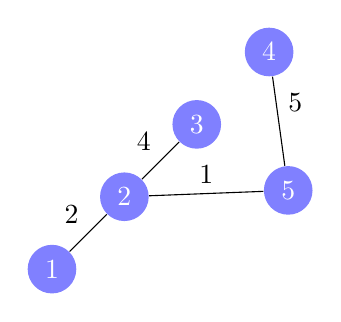
\begin{tikzpicture} 
            \node (node 1) [circle, double, double distance =1.2pt,text=white,fill=blue!50,] {1};
            \node (node 2) [circle, double, double distance =1.2pt,text=white,fill=blue!50,above right of= node 1] {2};
            \node (node 3) [circle, double, double distance =1.2pt,text=white,fill=blue!50,above right of= node 2] {3};
            \node (node 4) [circle, double, double distance =1.2pt,text=white,fill=blue!50,above right of= node 3] {4};
            \node (node 5) at(3, 1) [circle, double, double distance =1.2pt,text=white,fill=blue!50] {5};
            
            \path (node 1) edge[-,"2",] (node 2)
                  (node 2) edge[-,"4",] (node 3)
                  (node 2) edge[-,"1",] (node 5)
                  (node 4) edge[-,"5",] (node 5);
        \end{tikzpicture}
    %\end{center}
\end{document}
